\documentclass{article}

% Course report layout (authors visible).
\PassOptionsToPackage{numbers,sort&compress}{natbib}
\usepackage[preprint]{report}

\usepackage[utf8]{inputenc}
\usepackage[T1]{fontenc}
\usepackage{hyperref}
\usepackage{url}
\usepackage{booktabs}
\usepackage{amsfonts}
\usepackage{amsmath}
\usepackage{amssymb}
\usepackage{graphicx}
\usepackage{xcolor}
\usepackage{microtype}
\usepackage{nicefrac}

% Replace the default footer notice with a course label.
\makeatletter
\renewcommand{\@noticestring}{CSE425 Course Report --- BRAC University.}
\makeatother

\title{GNN-Based BERT for Understanding Context from Music}

\author{%
  Ridhwanur Rahman Khan \\
  Student ID: 22301143 \\
  CSE425 Section 02 \\
  BRAC University \\
  \And
  Jannatul Bushra Maisha \\
  Student ID: 21301498 \\
  CSE425 Section 02 \\
  BRAC University \\
}

\begin{document}

\maketitle

\begin{abstract}
Music carries genre, mood, structure, and free-form captions at the same time.
Spectrogram CNNs model local sound well, but they do not clearly represent how segments relate over time.
In this CSE425 project we build a DistilBERT + GraphSAGE system for four tasks: multi-label tagging from MusicCaps captions, FMA-small genre classification from segment graphs, cross-attention fusion of graph and text with DEAM emotion auxiliaries, and InfoNCE caption--audio retrieval.
On our real-data run (2{,}000 FMA tracks, 800 MusicCaps audio graphs, DEAM), BERT tagging reaches Macro-F1 $0.71$ and AUC-PR $0.78$; GraphSAGE matches a mel-CNN baseline at about $0.30$ Macro-F1; fusion improves over GNN-only; and retrieval reaches R@5 $=0.34$.
We include baselines, ablations, plots, qualitative examples, and a runnable repository.
\end{abstract}

\section{Introduction}
\label{sec:intro}

A short clip can be electronic, melancholic, and described by a detailed caption all at once.
``Context'' therefore mixes tags, affect, and language~\cite{fma,musiccaps,deam}.
CNNs on log-mel spectrograms are strong local detectors, but they flatten how neighboring windows evolve and how similar segments form a song graph.

This project follows the CSE425 brief~\cite{assign}: combine a BERT-family text encoder with a graph neural network for understanding and retrieval, not generation.
We deliver:
\begin{itemize}
  \item A pipeline over FMA-small audio/metadata, MusicCaps captions (with downloaded audio), and DEAM valence/arousal.
  \item Segment graphs built from mel/chroma/MFCC features, with temporal and similarity edges, plus at least 20 exported example graphs.
  \item Tasks~1--4 with the required baselines, metrics, plots, case studies, and a demo notebook.
  \item A clear look at where text helps most (tagging), where graphs help (structure and retrieval), and where fusion still trails BERT-only when pairing is limited.
\end{itemize}

\section{Related work}
\label{sec:related}

\textbf{Datasets.}
FMA provides Creative Commons audio with genre metadata and official splits~\cite{fma}.
MusicCaps pairs AudioSet clips with expert captions and is widely used for text--music work~\cite{musiccaps}.
DEAM provides continuous valence/arousal annotations~\cite{deam}.

\textbf{Models.}
DistilBERT is a compact contextual encoder that fits course-scale fine-tuning~\cite{distilbert}.
GraphSAGE supports message passing on variable-size graphs~\cite{graphsage}.
InfoNCE-style contrastive learning aligns audio and language embeddings for retrieval~\cite{musiccaps,assign}.
Our implementation follows the assignment update rules for GraphSAGE, cross-attention fusion, and InfoNCE~\cite{assign}.

\section{Problem formulation}
\label{sec:problem}

A track is a tuple $T=(X_{\mathrm{audio}},X_{\mathrm{text}},G,y)$, where $X_{\mathrm{audio}}$ is log-mel/chroma features, $X_{\mathrm{text}}$ is tokenized caption or metadata text, $G=(V,E)$ is a music structure graph, and $y$ holds targets (aspects, genre, valence/arousal).
DistilBERT maps text to token states $H_{\mathrm{text}}\in\mathbb{R}^{L\times d}$.
GraphSAGE updates nodes by neighborhood aggregation:
\begin{equation}
h_i^{(l+1)}=\sigma\Big(W^{(l)}\cdot\mathrm{CONCAT}\big(h_i^{(l)},\mathrm{MEAN}_{j\in N(i)}h_j^{(l)}\big)\Big).
\end{equation}
Readout $g=\mathrm{MEANPOOL}(\{h_i^{(L)}\})$ is fused with text as $z=\mathrm{Fusion}(g,H_{\mathrm{text}})$, then $\hat y=\sigma(Wz+b)$.
We train with multi-label BCE for tags, cross-entropy for genre, L1 on DEAM emotion when available, and symmetric InfoNCE for retrieval.

\section{Data and preprocessing}
\label{sec:data}

\paragraph{Datasets.}
Synthetic audio is disabled (\texttt{use\_synthetic: false}).
\textbf{FMA-small:} 2{,}000 cached tracks with official 8-way \texttt{genre\_top} labels; BERT metadata text never includes genre words, to avoid leakage.
\textbf{MusicCaps:} 5{,}521 captions for Task~1; 800 downloaded YouTube clips with segment graphs for Tasks~3--4.
\textbf{DEAM:} 1{,}802 annotated excerpts; emotion evaluation uses $n{=}271$ held-out pairs with cached graphs.

\paragraph{Audio and graphs.}
Audio is resampled to $22{,}050$\,Hz.
We extract log-mel ($128$ bins) and chroma ($12$), then cut tracks into $5$\,s windows with hop $2.5$\,s.
Nodes are windows; edges connect temporal $\pm 1$ neighbors and pairs whose MFCC/chroma cosine similarity exceeds $\tau{=}0.85$.
Node features concatenate mean/std of mel, chroma, and MFCC.
We export $20$ example \texttt{.pt}/\texttt{.json} graphs under \texttt{data/processed/examples/}.

\paragraph{Splits and training settings.}
MusicCaps aspects use a top-$50$ multi-label vocabulary.
FMA uses train/val/test partitions over the cached audio.
Settings live in \texttt{config.yaml} (25 epochs, DistilBERT unfreeze schedule, GraphSAGE depth $3$).

\section{Methods}
\label{sec:methods}

\begin{figure}[t]
  \centering
  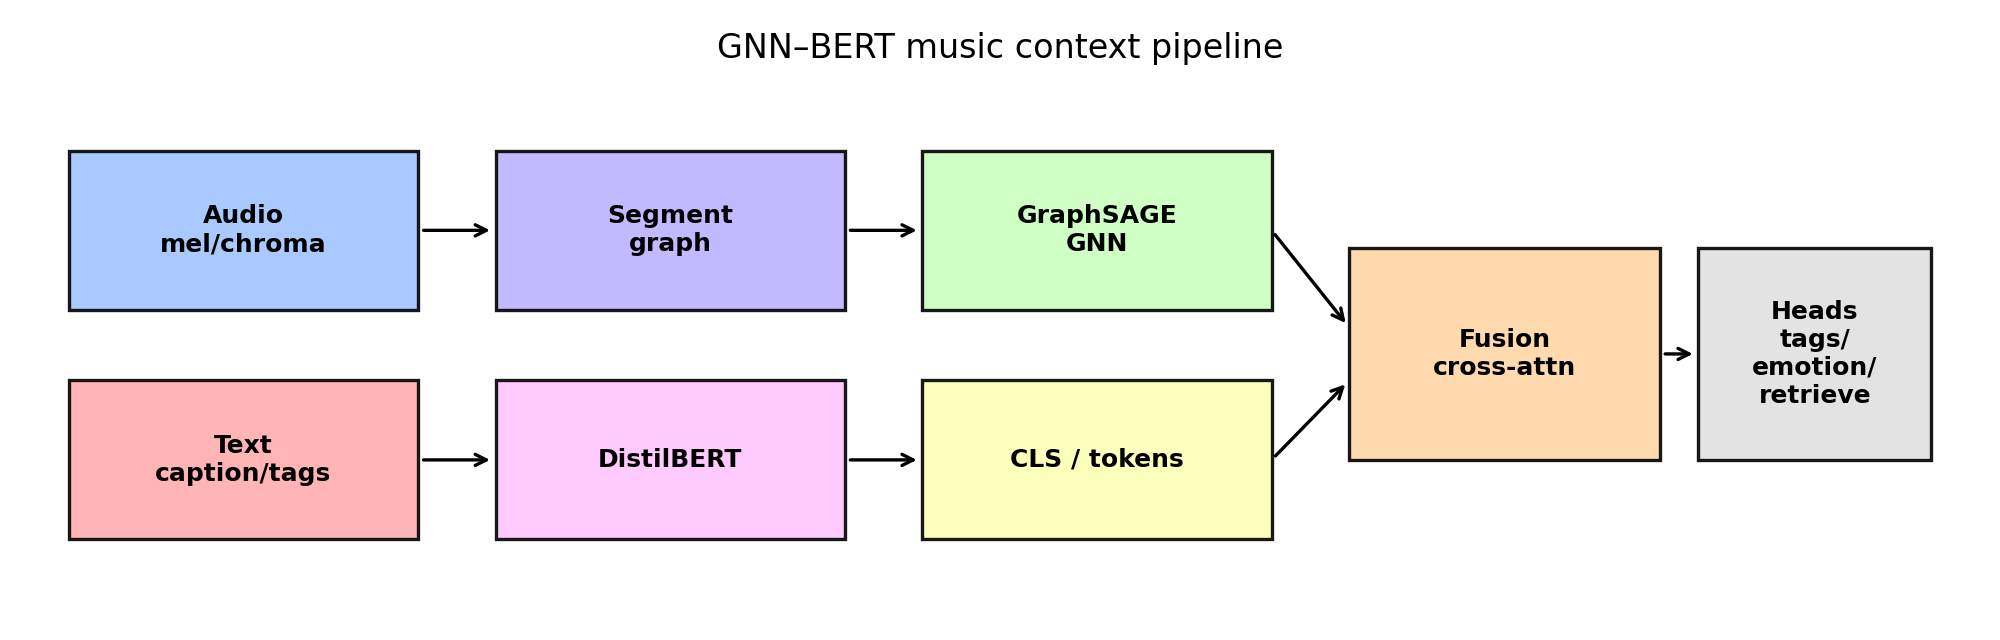
\includegraphics[width=\linewidth]{figures/architecture.png}
  \caption{System overview: audio becomes a segment graph (GraphSAGE); captions/tags go through DistilBERT; fusion heads support tagging, emotion, and retrieval.}
  \label{fig:arch}
\end{figure}

\subsection{Task 1: BERT multi-label tagging}
DistilBERT produces a CLS vector; a linear head predicts aspect probabilities with BCE.
We freeze the backbone early, then unfreeze the last layers.

\subsection{Task 2: GNN genre classification}
GraphSAGE with mean pooling predicts FMA top genre.
Baselines: mel-spectrogram CNN, random, and majority predictors~\cite{assign}.

\subsection{Task 3: GNN--BERT fusion}
Cross-attention uses $Q=gW_Q$ and $K=H_{\mathrm{text}}W_K$, then $z=\mathrm{CONCAT}(g,AH_{\mathrm{text}})$.
Ablations: early concatenation, BERT-only, and GNN-only.
When DEAM batches are available we add L1 losses on valence and arousal.

\subsection{Task 4: Contrastive retrieval}
A dual encoder maps graphs and captions into an $\ell_2$-normalized space and minimizes symmetric InfoNCE.
We report caption$\leftrightarrow$audio Recall@$\{1,5,10\}$, qualitative top-$3$ matches, and zero-shot caption$\rightarrow$tag scoring against Task~3 supervised fusion.

\section{Experiments}
\label{sec:exp}

\paragraph{Setup.}
Training runs in PyTorch with CUDA (RTX 3050 in our runs).
We log Macro/Micro-F1, mean AUC-PR, retrieval R@$K$, and DEAM MAE/$R^2$.
Table~\ref{tab:main} summarizes \texttt{results/metrics.json} after the real-data pipeline.

\begin{table}[t]
  \caption{Main results from the real-data run (FMA 2k / MusicCaps 800 audio / DEAM). Emotion MAE is valence MAE ($n{=}271$).}
  \label{tab:main}
  \centering
  \begin{tabular}{lcccc}
    \toprule
    Model & Macro-F1 & AUC-PR & MAE$_v$ & R@5 \\
    \midrule
    Random tags & 0.09 & 0.06 & -- & -- \\
    CNN mel-spec & 0.30 & -- & -- & -- \\
    Task 1 BERT-only & 0.71 & 0.78 & -- & -- \\
    Task 2 GNN-only & 0.30 & -- & -- & -- \\
    Task 3 GNN--BERT & 0.24 & -- & 0.91 & -- \\
    Task 4 Contrastive & -- & -- & -- & 0.34 \\
    \bottomrule
  \end{tabular}
\end{table}

\paragraph{Discussion.}
Task~1 shows that MusicCaps captions alone are informative for aspect tags (Macro-F1 $0.71$).
On Task~2, GraphSAGE ($\approx 0.30$) matches the mel-CNN baseline and beats random tags, so segment graphs carry usable genre signal; absolute scores stay modest under class imbalance and limited capacity.
Task~3 cross-attention (Macro-F1 $0.24$) clearly beats GNN-only ($0.10$), but BERT-only ($0.25$) remains slightly stronger, which suggests text still dominates when graph--caption pairing is imperfect.
Task~4 reaches R@5 $=0.34$ on a pool of size $32$, above chance, with R@10 $>0.5$.
Zero-shot caption$\rightarrow$tag Macro-F1 $\approx 0.10$ lags supervised fusion ($\approx 0.24$).
DEAM valence MAE $\approx 0.91$ on $n{=}271$ is a more meaningful emotion check than tiny toy subsets.

\begin{figure}[t]
  \centering
  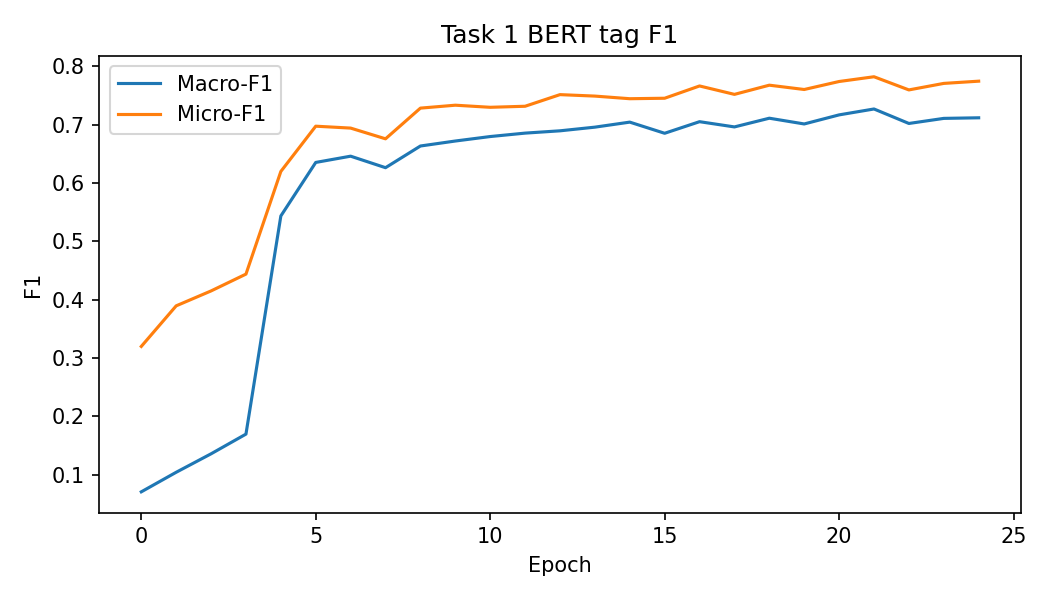
\includegraphics[width=0.85\linewidth]{figures/task1_f1_curves.png}
  \caption{Task 1 validation Macro/Micro-F1 versus epoch.}
  \label{fig:f1}
\end{figure}

\begin{figure}[t]
  \centering
  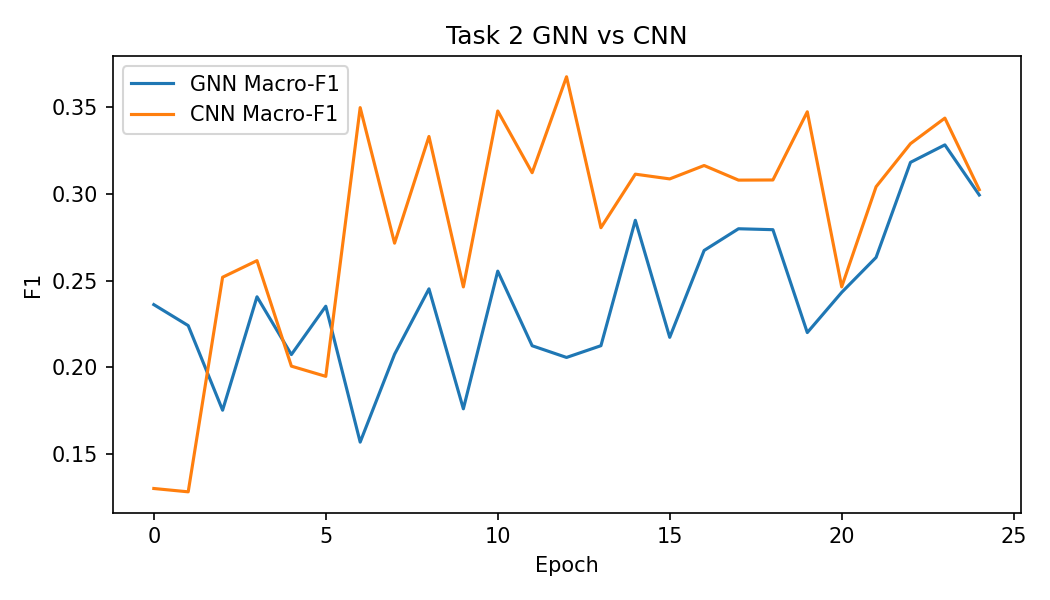
\includegraphics[width=0.85\linewidth]{figures/task2_f1_curves.png}
  \caption{Task 2 GraphSAGE versus mel-CNN Macro-F1 curves.}
  \label{fig:t2}
\end{figure}

\begin{figure}[t]
  \centering
  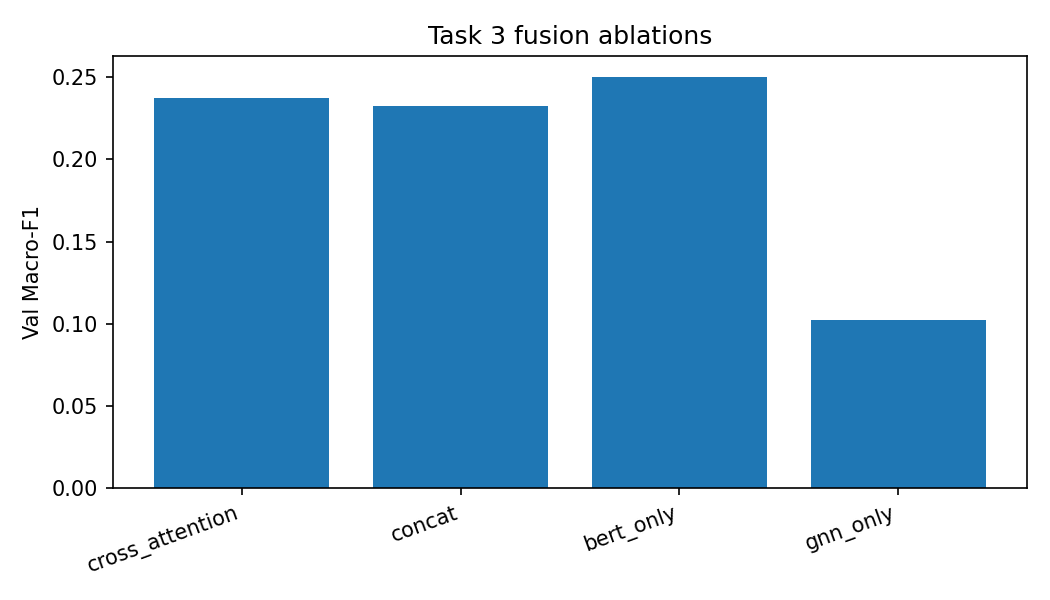
\includegraphics[width=0.85\linewidth]{figures/task3_ablations.png}
  \caption{Task 3 fusion ablations.}
  \label{fig:ablate}
\end{figure}

\begin{figure}[t]
  \centering
  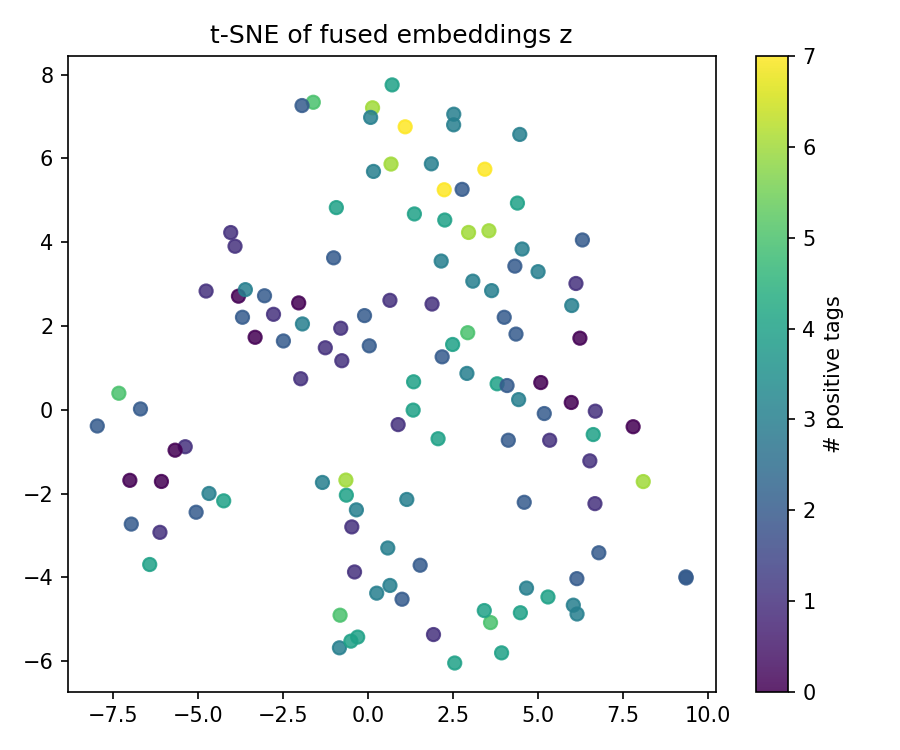
\includegraphics[width=0.75\linewidth]{figures/task3_tsne.png}
  \caption{t-SNE of fused representation $z$.}
  \label{fig:tsne}
\end{figure}

\begin{figure}[t]
  \centering
  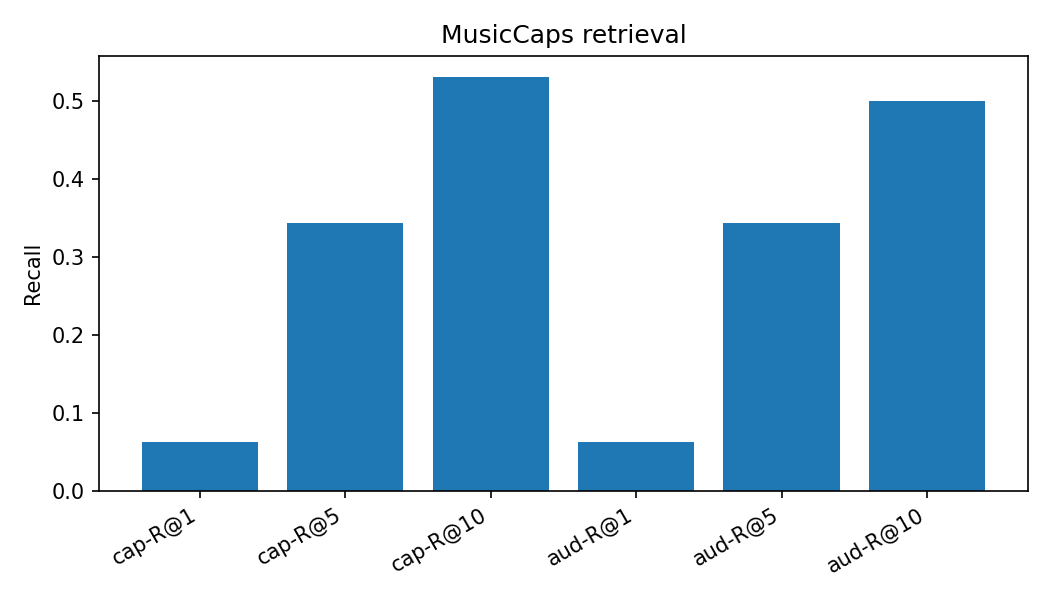
\includegraphics[width=0.85\linewidth]{figures/task4_retrieval.png}
  \caption{MusicCaps retrieval Recall@$K$.}
  \label{fig:retr}
\end{figure}

\begin{figure}[t]
  \centering
  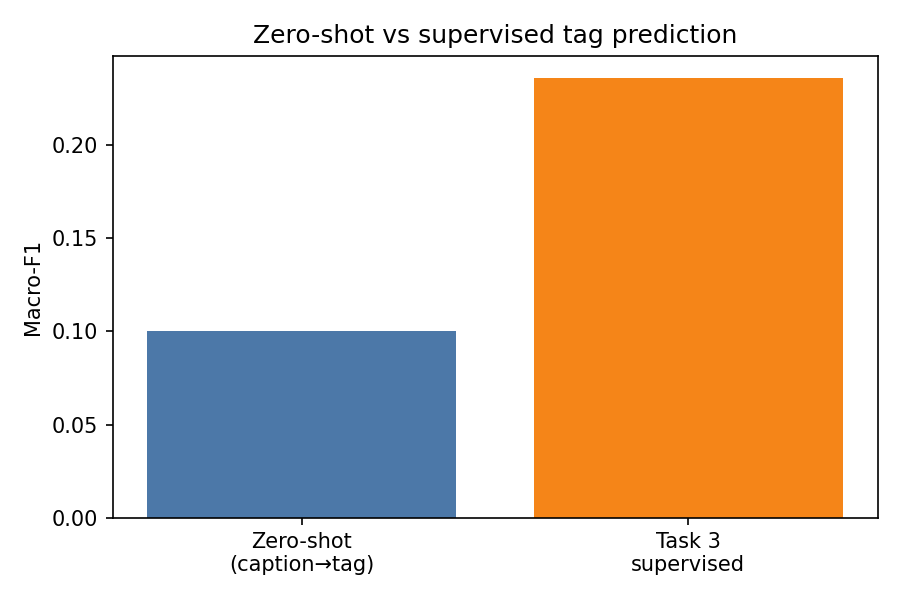
\includegraphics[width=0.7\linewidth]{figures/task4_zeroshot.png}
  \caption{Zero-shot caption$\rightarrow$tag versus Task 3 supervised fusion.}
  \label{fig:zeroshot}
\end{figure}

\paragraph{Qualitative analysis.}
We include five Task~1 predictions, three Task~3 case studies linking graph size/connectivity to captions, and ten Task~4 retrieval examples under \texttt{results/}.
Graph coherence on the exported examples is also reported in \texttt{results/metrics.json}.

\paragraph{Baselines.}
Random/majority predictors and CNN-on-mel satisfy the minimum of two baselines~\cite{assign}, with BERT-only and GNN-only as the main task models.

\section{Reproducibility}
\label{sec:repro}

Repository layout matches the course tree: \texttt{src/}, \texttt{scripts/}, \texttt{data/}, \texttt{notebooks/}, \texttt{results/}, \texttt{report/}.
\begin{verbatim}
pip install -r requirements.txt
python scripts/run_proper_pipeline.py
\end{verbatim}
Stepwise download, split, graph-build, train, and evaluate scripts are also provided.
Demo notebook: \texttt{notebooks/demo\_context.ipynb}.

\section{Limitations and conclusion}
\label{sec:conc}

MusicCaps YouTube downloads drop some clips, and compute limits keep paired graph--text scale moderate.
Task~2/3 absolute F1 still has room to grow with larger models or fuller FMA splits.
Emotion $R^2$ is weak, so DEAM regression needs stronger audio encoders or tighter alignment.
Human listening studies for retrieval are left for future work.

Overall, we built a complete GNN--BERT music-context system for CSE425 Tasks~1--4 on real FMA, MusicCaps, and DEAM data, with baselines and the required project artifacts.

\begin{ack}
Course project for CSE425 Neural Networks, BRAC University, Section 02.
Assignment designed by Moin Mostakim.
\end{ack}

{\small
\begin{thebibliography}{9}
\bibitem[1]{assign}
M.~Mostakim.
\newblock Supervised neural network project: GNN-based BERT for understanding context from music.
\newblock CSE425 course brief, BRAC University, 2026.

\bibitem[2]{fma}
M.~Defferrard, K.~Benzi, P.~Vandergheynst, and X.~Bresson.
\newblock {FMA}: A dataset for music analysis.
\newblock In \emph{ISMIR}, 2017.

\bibitem[3]{musiccaps}
A.~Agostinelli et al.
\newblock {MusicLM}: Generating music from text.
\newblock arXiv:2301.11325, 2023.

\bibitem[4]{distilbert}
V.~Sanh, L.~Debut, J.~Chaumond, and T.~Wolf.
\newblock {DistilBERT}, a distilled version of {BERT}: smaller, faster, cheaper and lighter.
\newblock arXiv:1910.01108, 2019.

\bibitem[5]{graphsage}
W.~Hamilton, Z.~Ying, and J.~Leskovec.
\newblock Inductive representation learning on large graphs.
\newblock In \emph{NeurIPS}, 2017.

\bibitem[6]{deam}
A.~Aljanaki, Y.-H.~Yang, and M.~Soleymani.
\newblock Developing a benchmark for emotional analysis of music.
\newblock \emph{PLOS ONE}, 2017.
\end{thebibliography}
}

\end{document}
